% =============================================================================
% KAPITEL 4: AUSWERTUNG UND DISKUSSION
% =============================================================================

\section{Auswertung und Diskussion}
\label{sec:auswertung_diskussion}

Dieses Kapitel widmet sich der Untersuchung, wie verschiedene Leitergeometrien die Messgenauigkeit der Stromwandler beeinflussen. Der Schwerpunkt liegt zunächst auf der allgemeinen Einwirkung durch die Anordnung. Im Anschluss folgen eine detaillierte Analyse der einzelnen Außenleiter sowie eine ökonomische Bewertung der Resultate.

\subsection{Einfluss der Leitergeometrie auf die Messgenauigkeit}
\label{sec:einfluss_leitergeometrie}

Die folgenden Diagramme visualisieren die Messabweichungen der Stromwandler in Abhängigkeit vom Primärstrom sowie der Leiteranordnung. Der Vergleich erfolgt jeweils zwischen Wandlern mit identischem Nennstrom. Eine genaue Beschreibung der verwendeten Leiteranordnungen findet sich in Abschnitt \ref{sec:layout_geometrie}.

Zur visuellen Unterscheidung gelten in den Diagrammen folgende Konventionen
\begin{itemize}
    \item Die \textbf{Parallelanordnung} wird durch eine durchgezogene Linie in Kombination mit einem Kreissymbol dargestellt
    \item Die \textbf{Dreiecksanordnung} ist durch eine gepunktete oder gestrichelte Linie sowie ein Dreieckssymbol gekennzeichnet
    \item Die \textbf{Farbgebung} verbleibt für ein spezifisches Wandlermodell in beiden Anordnungen gleich um den direkten Vergleich zu ermöglichen
\end{itemize}
Diese Darstellungsweise erlaubt die direkte Bewertung des Geometrieeinflusses auf den jeweiligen Wandlertyp.


% --- Hier beginnt der neue Unterabschnitt für den besseren Übergang ---
\subsubsection{Referenzanalyse bei \SI{2000}{A} Einfluss der Leitergeometrie auf verschiedene Wandlerkonzepte}
\label{sec:analyse_messreihe_2000A}

Die Untersuchung der Stromwandler bei einem Nennstrom von \SI{2000}{A} liefert differenzierte Ergebnisse für die verschiedenen Modelle und Leiteranordnungen. Abbildung \ref{dia:2000A_zusammenfassung} stellt die Verläufe der vier Prüflinge gegenüber und verdeutlicht die Einhaltung der Genauigkeitsklasse 1 für den Großteil der Messpunkte. Der grafische Vergleich hebt hervor dass insbesondere zwei Konfigurationen erkennbare Abweichungen aufweisen. Dies betrifft den Redur 13A1030.ffp in der Dreiecksanordnung sowie den Celsa ALO 10030 in der Parallelanordnung. Beide Wandler verlassen in diesen spezifischen Szenarien die vorgegebenen Toleranzbereiche.

\begin{diagram}[H]
    \centering
    \includegraphics[width=1.0\textwidth]{03_Ressourcen/diagramme/dia_2000A_dreieck_parallel/dia_2000A_dreieck_parallel-Zusammenfassung_MultiCurrent.pdf}
    \caption{Zusammenfassender Vergleich der Leitergeometrien bei \SI{2000}{A}}
    \label{dia:2000A_zusammenfassung}
\end{diagram}

Eine bauliche Besonderheit weist der Redur 13A1030.ffp auf. Wie in Abbildung \ref{fig:wandler_fremdfeldprotektor} zu erkennen ist befinden sich die Fremdfeldprotektoren (\gls{ffp}) an den seitlichen Flanken des Gehäuses. Diese Positionierung schirmt den Eisenkern gegen magnetische Streufelder benachbarter Leiter ab sofern diese seitlich angeordnet sind. In der parallelen Leiterführung resultiert dies in normkonformen Messergebnissen da die Beeinflussung durch die Nachbarphasen minimiert wird.

\begin{figure}[H]
    \centering
    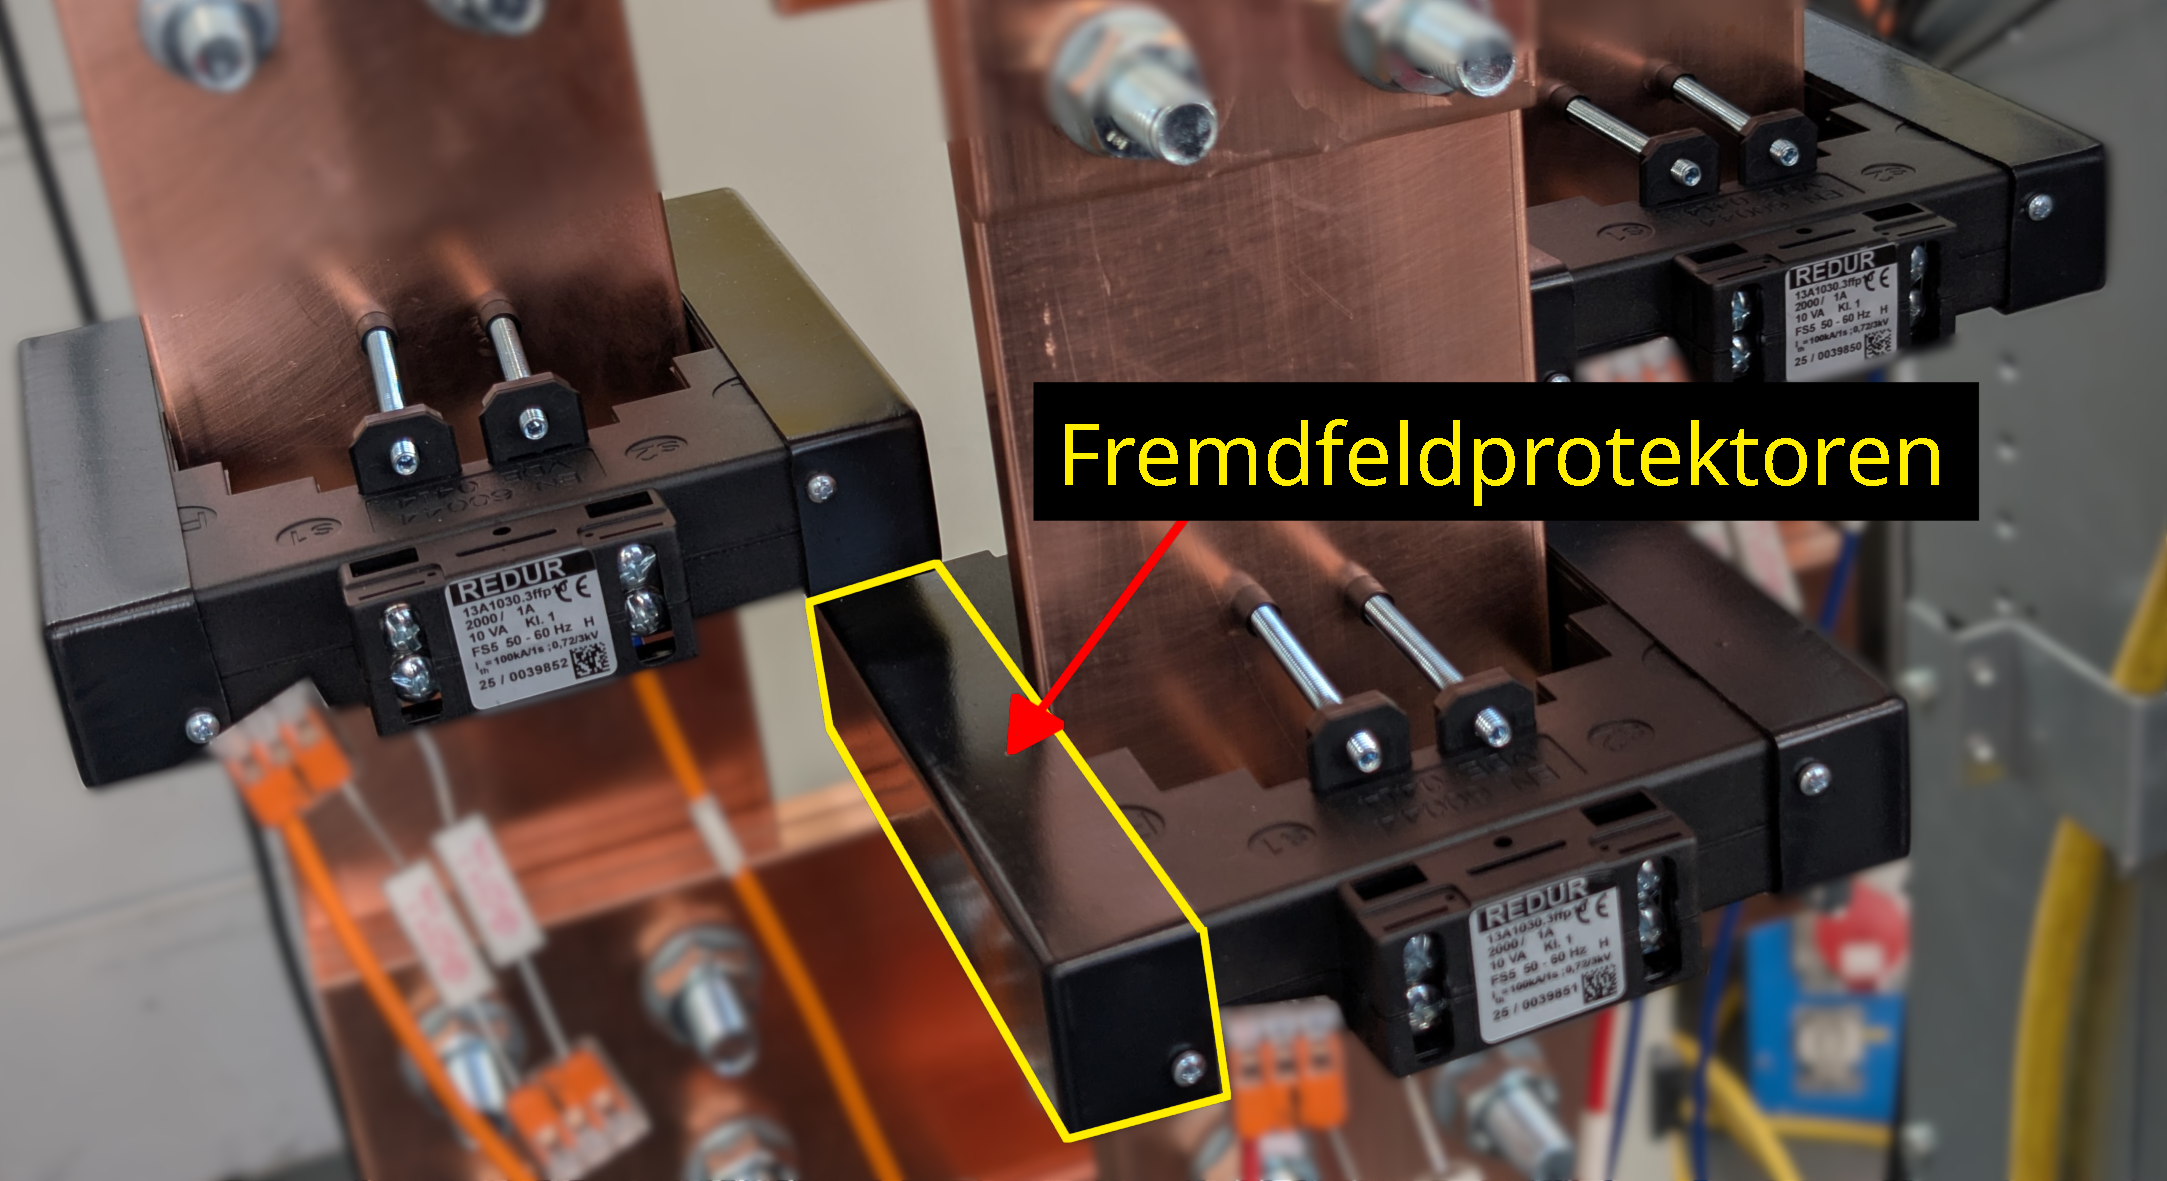
\includegraphics[width=0.8\textwidth]{03_Ressourcen/Bilder/wandler_redur_2000A_dreiecksmessung_beschriftet.pdf}
    \caption{Seitliche Fremdfeldprotektoren am Redur Wandler}
    \label{fig:wandler_fremdfeldprotektor}
\end{figure}

Die Grenzen dieser Schirmungstechnologie offenbaren sich in der Dreiecksanordnung. Die detaillierten numerischen Ergebnisse für diesen Aufbau sind in Tabelle \ref{tab:messergebnisse_redur_2000A} im Anhang zu finden. Die Phase L2 weist bei \SI{120}{\%} des Nennstroms eine Abweichung von \SI{-1,5}{\%} auf. Dieser Wert liegt außerhalb der zulässigen Toleranz der Genauigkeitsklasse 1. Ursächlich hierfür ist die fehlende magnetische Schirmung auf der Rückseite des Wandlergehäuses. In der Dreiecksgeometrie können die Magnetfelder der benachbarten Leiter an dieser ungeschützten Stelle in den Eisenkern eindringen und sättigen diesen partiell. Im Gegensatz dazu bleibt die Phase L1 mit einer Abweichung von lediglich \SI{-0,1}{\%} im selben Lastpunkt weit innerhalb der Normgrenzen.

Ein konträres Verhalten ist beim Modell Celsa ALO 10030 zu beobachten. Tabelle \ref{tab:messergebnisse_celsa_2000A} im Anhang dokumentiert die Messergebnisse für diesen Wandler und belegt substanzielle Einbußen der Genauigkeit in der parallelen Leiteranordnung. Bereits bei Nennstrom verletzt die Phase L2 mit \SI{-2,0}{\%} den zulässigen Grenzwert. Bei einer Überlast von \SI{120}{\%} steigt die Abweichung weiter auf \SI{-4,2}{\%} an. Auch die Außenleiter L1 und L3 zeigen in der Parallelanordnung bei \SI{120}{\%} Last mit Werten von \SI{-2,7}{\%} beziehungsweise \SI{-3,1}{\%} erkennbare Fehler. Die Änderung der Geometrie hin zur Dreiecksanordnung bewirkt bei diesem Modell eine Verbesserung. Der Fehler der Phase L2 reduziert sich hierbei bei \SI{120}{\%} Last auf einen unkritischen Wert von \SI{-0,2}{\%}.

Diese Abhängigkeit des Fehlers vom Primärstrom wird in Abbildung \ref{dia:2000A_celsa_zusammenfassung} grafisch aufbereitet. Das Diagramm veranschaulicht den steilen Abfall der Messkurven für die Parallelanordnung ab etwa \SI{20}{\%} des Nennstroms. Im Vergleich dazu verlaufen die Kurven der Dreiecksanordnung weitestgehend linear und verbleiben im Toleranzbereich.

\begin{diagram}[H]
    \centering
    \includegraphics[width=1.0\textwidth]{03_Ressourcen/diagramme/dia_2000A_celsa_10030/dia_2000A_celsa_10030-Zusammenfassung_MultiCurrent.pdf}
    \caption{Messfehlerverlauf des Celsa ALO 10030 in Abhängigkeit vom Primärstrom}
    \label{dia:2000A_celsa_zusammenfassung}
\end{diagram}

Im Gegensatz zu den Abweichungen der vorangegangenen Modelle zeigen der Celsa ALO 8030 K und der MBS ASK101.4 eine hohe Stabilität gegenüber externen Feldern. Diese Unempfindlichkeit lässt sich beim Celsa ALO 8030 K auf die Bauweise als kompensierter Wandler zurückführen wie in Abschnitt \ref{sec:kompensationswicklungen} erläutert wird. Tabelle \ref{tab:messergebnisse_celsa8030_2000A} im Anhang fasst die Ergebnisse für dieses Modell zusammen. Selbst unter Volllast und Überstrom bleiben alle Phasen in beiden geometrischen Anordnungen sicher innerhalb der Klasse 1. Die maximale Abweichung tritt in der Parallelanordnung bei Phase L1 mit einem Wert von \SI{-0,4}{\%} auf.

Ein ähnlich robustes Verhalten bestätigt Tabelle \ref{tab:messergebnisse_mbs_2000A} im Anhang für den MBS ASK101.4. Auch hier sind keine signifikanten Einflüsse durch die Leiteranordnung erkennbar. Die Messwerte liegen konstant auf einem Niveau vergleichbar mit dem Celsa 8030 K. In der Dreiecksanordnung erreicht die Phase L1 bei \SI{120}{\%} Last beispielsweise eine Abweichung von \SI{-0,3}{\%} und demonstriert damit die Unempfindlichkeit dieses Modells gegenüber den untersuchten geometrischen Anordnungen.


\subsubsection{Einfluss der Leitergeometrie auf das Sättigungsverhalten bei \SI{2500}{A}}
\label{sec:analyse_messreihe_2500A}

Die Analyse der Messreihe bei \SI{2500}{A} verdeutlicht den Einfluss der Leitergeometrie auf unterschiedliche Wandlertechnologien. Im Fokus steht der Vergleich zwischen dem kompensierten Wandler Celsa ALO 10050 K und dem Standardwandler Celsa ALO 10030 in Bezug auf ihre Stabilität in Parallel- und Dreiecksanordnungen.

\begin{aufgabenbox}
    Hier möchte ich noch eine Simulation machen.
    Es sollen die Sättigungseffekte des Eisenkernes betrachet werden.
\end{aufgabenbox}

\begin{diagram}[H]
    \centering
    \includegraphics[width=1.0\textwidth]{03_Ressourcen/diagramme/dia_2500A_dreieck_parallel/dia_2500A_dreieck_parallel-Zusammenfassung_MultiCurrent.pdf}
    \caption{Zusammenfassender Vergleich der Leitergeometrien bei \SI{2500}{A}}
    \label{dia:2500A_zusammenfassung}
\end{diagram}

Die Messergebnisse des kompensierten Wandlers Celsa ALO 10050 K belegen dass dieser über den Großteil des Messbereichs eine hohe Genauigkeit aufweist (siehe Tabelle \ref{tab:messergebnisse_celsa10050_2500A_alle} im Anhang). In der Parallelanordnung bewegt sich der Wandler fast durchgehend innerhalb der Normvorgaben. Eine Ausnahme bildet die Phase L2 im Überlastbereich (\SI{120}{\%} $I_n$). Hier überschreitet der Wandler den Grenzwert mit einer Abweichung von rund \SI{-1,0}{\%} knapp was einem absoluten Fehlstrom von rund \SI{30}{A} entspricht. In der Dreiecksanordnung reduziert sich dieser Messfehler auf etwa \SI{-0,55}{\%} wodurch die Norm wieder eingehalten wird. Dies zeigt dass selbst ein kompensierter Wandler nicht vollständig immun gegen externe Magnetfelder ist die Auswirkungen jedoch im Vergleich zu Standardwandlern gering bleiben. Da sich der Fehlerbetrag hierbei fast halbiert führt die Dreiecksgeometrie in diesem kritischen Lastpunkt zu einer annähernden Verdopplung der Messgenauigkeit.

Im Gegensatz dazu zeigt der nicht kompensierte Standardwandler Celsa ALO 10030 in beiden Anordnungen erhebliche Abweichungen die auf eine magnetische Sättigung hindeuten (siehe Tabelle \ref{tab:messergebnisse_celsa10030_2500A_alle} im Anhang). In der Parallelanordnung steigt der Fehler bereits ab \SI{50}{\%} Nennstrom erkennbar an. Bei \SI{100}{\%} Last liegen die Abweichungen zwischen \SI{-10}{\%} und \SI{-16}{\%}.
Um das Ausmaß dieser Sättigungseffekte im Hochlastbereich zu verdeutlichen stellt Tabelle \ref{tab:vergleich_hochstlast_celsa_extended} die absoluten Fehlströme der Phase L2 gegenüber und quantifiziert den Gewinn durch die geometrische Optimierung.

\begin{table}[htbp]
    \centering
    \caption{Vergleich der Fehlströme und Genauigkeitsgewinn (Celsa ALO 10030, Phase L2)}
    \label{tab:vergleich_hochstlast_celsa_extended}
    \small
    \begin{tabular}{
            l
            S[table-format=4.0]
            S[table-format=2.2]
            S[table-format=3.2]
            S[table-format=2.1]
        }
        \toprule
        {Lastpunkt}  & {Primärstrom} & {Fehlstrom Dreieck} & {Fehlstrom Parallel} & {Verbesserung} \\
        {[\% $I_n$]} & {[A]}         & {[A]}               & {[A]}                & {[\%]}         \\
        \midrule
        80           & 2000          & 31.35               & 231.42               & 10.0           \\
        90           & 2250          & 39.67               & 321.22               & 12.5           \\
        100          & 2500          & 45.85               & 415.59               & 14.8           \\
        120          & 3000          & 58.49               & 616.96               & 18.6           \\
        \bottomrule
    \end{tabular}
\end{table}


Wie den Werten zu entnehmen ist bricht die Genauigkeit im Überlastbereich bei \SI{120}{\%} ein. Während in der Parallelanordnung ein Fehlstrom von über \SI{600}{A} auftritt sinkt dieser in der Dreiecksanordnung auf rund \SI{58}{A}. Dies entspricht einer Verbesserung der Genauigkeit um \num{18,6} Prozentpunkte. Auch die Phasen L1 und L3 liegen in der Parallelanordnung mit \SI{-16,2}{\%} beziehungsweise \SI{-13,9}{\%} weit außerhalb der Toleranzgrenzen profitieren jedoch in ähnlichem Maße von der Umstellung auf die Dreiecksgeometrie.

Dennoch muss konstatiert werden dass selbst die optimierte Dreiecksanordnung nicht ausreicht um die normativen Vorgaben zu erfüllen. Trotz der Fehlerminimierung verbleibt der Wandler außerhalb der Genauigkeitsklasse 1.

Diese verbleibende Abweichung deutet auf eine grundsätzliche Unterdimensionierung des magnetischen Kreises hin. Ein Vergleich mit den Ergebnissen aus Abschnitt \ref{sec:analyse_messreihe_2000A} stützt diese Hypothese da bereits dort der Wandlertyp Sättigungstendenzen im Nennstrombereich zeigte.
Bei dem hier untersuchten \SI{2500}{A}-Modell wird anhand von Tabelle \ref{tab:vergleich_hochstlast_celsa_extended} ersichtlich dass der Fehleranstieg bereits bei \SI{80}{\%} der Nennlast einsetzt. Dies entspricht einem Primärstrom von \SI{2000}{A}.

Damit korreliert der Sättigungsbeginn exakt mit den Beobachtungen der vorherigen Messreihe. Dies lässt den Schluss zu dass das physikalische Eisenkernvolumen dieses Bauteils unabhängig von der Nennstromangabe auf dem Typenschild für Ströme oberhalb von \SI{2000}{A} nicht ausreichend dimensioniert ist.

Dieser empirische Befund bestätigt die theoretischen Zusammenhänge die durch Gleichung \ref{eq:b_phi_relation} in Abschnitt \ref{sec:theorie_fremdfelder} beschrieben werden. Wie dort hergeleitet führt der geringe Eisenquerschnitt $A$ des kleinen Wandlers dazu dass sich der magnetische Fluss auf eine zu kleine Fläche konzentriert. Dies bewirkt trotz der absolut gesehen geringeren Störflussaufnahme einen kritischen Anstieg der resultierenden Flussdichte $B_{\text{res}}$ wodurch die Sättigungsgrenze des Materials frühzeitig erreicht wird.

Tabelle \ref{tab:wandler_volumen} untermauert diese Vermutung durch die Berechnung des effektiven Materialvolumens. Während der Typ ALO 10050 über ein Nettovolumen von \SI{623,6}{cm^3} verfügt weist der hier betrachtete ALO 10030 lediglich \SI{265,5}{cm^3} auf. Damit steht diesem Wandler weniger als die Hälfte des Volumens zur Verfügung was die frühe Sättigung physikalisch plausibilisiert.

\begin{table}[H]
    \centering
    \caption{Berechnetes Nettovolumen der untersuchten Wandler}
    \label{tab:wandler_volumen}
    \begin{tabular}{l c c S[table-format=3.1]}
        \toprule
        {Modell}    & {Gehäusemaße ($H \times B \times T$)} & {Fenstergeometrie}        & {Nettovolumen [\unit{cm^3}]} \\
        \midrule
        ALO 10030   & $31 \times 129 \times \SI{141}{mm}$   & $\varnothing$ \SI{55}{mm} & 265.5                        \\
        ALO 10050 K & $50 \times 130 \times \SI{141}{mm}$   & $50 \times \SI{101}{mm}$  & 623.6                        \\
        \bottomrule
    \end{tabular}
\end{table}

Einschränkend ist anzumerken dass das berechnete Volumen auf der Gehäusegeometrie basiert und nicht exakt dem Volumen des Eisenkerns entspricht. Da jedoch ein beachtlicher Unterschied im Volumenfaktor vorliegt ist der Vergleich als Näherung für die verfügbare Eisenkern zulässig.


Der Celsa ALO 10050 K dient an dieser Stelle lediglich als geometrische Referenzgröße. Es ist nicht zulässig die höhere Genauigkeit dieses Typs allein auf das größere Volumen zurückzuführen da dessen Messstabilität primär durch die Kompensationstechnik erreicht wird.



% --- 3000 A ---


\subsubsection{Einfluss von Geometrie und Bürde bei \SI{3000}{A}}
\label{sec:analyse_messreihe_3000A}

Die Messreihe bei einer Stromstärke von \SI{3000}{A} fungiert als zentrale Fallstudie um das Verhalten der Wandler im Grenzbereich ihrer Leistungsfähigkeit zu charakterisieren. Zentraler Gegenstand dieser Betrachtung ist der technologische Vergleich zwischen dem Standardwandler Celsa ALO 12070 und der kompensierten Ausführung ALO 12070 K unter dem Einfluss der Leitergeometrie. Ergänzend wird untersucht inwiefern eine Reduktion des sekundären Bürdenwiderstands die Sättigungseffekte in der kritischen Parallelanordnung abmildern kann.

\paragraph{Vergleich der Wandlertechnologien und Geometrien}

Abbildung \ref{dia:3000A_zusammenfassung} stellt die Fehlerverläufe beider Wandlertypen in Dreiecks- und Parallelanordnung gegenüber. 

Die Untersuchung des Standardwandlers ALO 12070 in der Parallelanordnung offenbart dass der Leiter L2 als einziger die Genauigkeitsanforderungen nicht erfüllen kann. Wie in Tabelle \ref{tab:messergebnisse_celsa12070_3000A_alle} im Anhang ersichtlich fällt der Messwert bereits bei \SI{80}{\%} des Nennstromes mit \SI{-1,1}{\%} unter den Grenzwert. Dieser Fehler verstärkt sich linear bis in den Überlastbereich wo er bei \SI{120}{\%} Last einen Wert von \SI{-5,4}{\%} erreicht was einem absoluten Fehlstrom von rund \SI{195,3}{A} entspricht.

Demgegenüber belegt der kompensierte Typ ALO 12070 K dass die zusätzliche Wicklung die Erfassung bei L2 stabilisiert und die Normeinhaltung gewährleistet. Im Überlastbereich ist in der Parallelanordnung eine Abweichung in den positiven Bereich zu beobachten was auf Effekte ähnlich einer Unterbürdung durch Flussveränderungen im Kern schließen lässt. Die Außenleiter L1 und L3 weisen hingegen in beiden Konfigurationen ein nahezu identisches Verhalten auf. Der direkte Vergleich der Geometrien beim kompensierten Wandler verdeutlicht den Vorteil der Dreiecksanordnung bei Phase L2 merklich. Der Fehler reduziert sich von \SI{0,9}{\%} in der Parallelanordnung auf \SI{0,1}{\%} in der Dreiecksanordnung was einer Verbesserung um den Faktor zehn gleichkommt.

\begin{diagram}[H]
    \centering
    \includegraphics[width=1.0\textwidth]{03_Ressourcen/diagramme/dia_3000A_dreieck_parallel/dia_3000A_dreieck_parallel-Zusammenfassung_MultiCurrent.pdf}
    \caption{Vergleich von Geometrie und Bürdeneinfluss bei \SI{3000}{A}}
    \label{dia:3000A_zusammenfassung}
\end{diagram}

\paragraph{Analyse der Bürdenabhängigkeit}

Da der Standardwandler in der Parallelanordnung erkennbare Sättigungserscheinungen zeigte wurde in einer vertiefenden Untersuchung analysiert ob eine Reduktion der sekundären Bürde diese Effekte kompensieren kann. Hierzu wurden drei Konfigurationen verglichen die Nennbürde (Referenzlast) der Betrieb ohne Vorwiderstand (Minimallast) und eine asymmetrische Belastung bei der nur der kritische Leiter L2 entlastet wurde (siehe Tabelle \ref{tab:buerden_konfigurationen_3000A}).

\begin{table}[H]
    \centering
    \caption{Übersicht der untersuchten Bürdenkonfigurationen bei \SI{3000}{A}}
    \label{tab:buerden_konfigurationen_3000A}
    \begin{tabular}{l c c c l}
        \toprule
                                   & \multicolumn{3}{c}{Bürdenwiderstand $R_B$ [\unit{\ohm}]} &                                        \\
        \cmidrule(lr){2-4}
        {Konfiguration}            & {L1}                                                     & {L2} & {L3} & {Ziel der Untersuchung}                  \\
        \midrule
        Referenzlast               & 10,8                                                     & 10,8 & 10,8 & Basisvergleich Geometrieeinfluss       \\
        Minimallast                & 0,0                                                      & 0,0  & 0,0  & Bestimmung maximaler Sättigungsgrenze  \\
        Asymmetrische Last & 10,8                                                     & 0,0  & 10,8 & Selektive Entlastung des Mittelleiters \\
        \bottomrule
    \end{tabular}
\end{table}

Abbildung \ref{dia:3000A_buerde_verlauf} visualisiert die Ergebnisse dieser Variation. Für die Außenleiter L1 und L3 ist kaum eine Abhängigkeit von der Bürde festzustellen da ihre Abweichungen im Nieder- und Nennstrombereich konstant gering bleiben. Anders stellt sich die Situation beim mittleren Leiter L2 dar.

\begin{diagram}[H]
    \centering
    \includegraphics[width=1.0\textwidth]{03_Ressourcen/diagramme/dia_3000A_buerde/dia_3000A_buerde-Zusammenfassung_MultiCurrent.pdf}
    \caption{Vergleich der Fehlerkurven bei variabler Bürde und \SI{3000}{A}}
    \label{dia:3000A_buerde_verlauf}
\end{diagram}

Ein Vergleich zwischen der Referenzlast (Tabelle \ref{tab:messergebnisse_celsa12070_3000A_alle} im Anhang) und der asymmetrischen Last (Tabelle \ref{tab:messergebnisse_celsa12070_3000A_asym} im Anhang) zeigt bei L2 ein nahezu identisches Verhalten da beide Konfigurationen stark sättigen. Während die asymmetrische Last bei \SI{100}{\%} des Nennstromes bei \SI{-3,0}{\%} liegt weist die Referenzlast mit \SI{-2,9}{\%} eine fast gleiche Abweichung auf was einer Differenz von lediglich \SI{0,1}{\%} entspricht. Auch im Überlastbereich bei \SI{120}{\%} bleiben die Werte vergleichbar da die asymmetrische Last hier \SI{-5,7}{\%} und die Referenzlast \SI{-5,4}{\%} erreicht.

Die Konfiguration der Minimallast (Tabelle \ref{tab:messergebnisse_celsa12070_3000A_min} im Anhang) erweist sich für den kritischen Leiter L2 als die stabilste Variante. Bei \SI{80}{\%} des Nennstromes liegt der Fehler von L2 hier bei nur \SI{-0,6}{\%} wohingegen die Referenzlast bereits auf \SI{-1,1}{\%} abfällt was eine Verbesserung von rund \SI{0,5}{\%} durch die minimale Bürde bedeutet. Dennoch reicht auch die Minimallast nicht aus um den Standardwandler in der Parallelanordnung bei Nennstrom in die Genauigkeitsklasse 1 zurückzuführen (\SI{-2,5}{\%} Abweichung).

Der Performance Index in Abbildung \ref{dia:3000A_performance_buerde} fasst die Ergebnisse zusammen. Zwar erzielt die Messung mit der Minimallast über alle Strombereiche hinweg die besten Ergebnisse doch zeigt der Vergleich mit dem vorangegangenen Abschnitt dass die Wahl der Wandlertechnologie (Kompensation) und der Geometrie (Dreieck) einen weitaus größeren Einfluss auf die Messgüte hat als die Optimierung der Bürde. Die Reduktion des Widerstands zögert die Sättigung physikalisch bedingt zwar hinaus kann die systembedingten Schwächen der Parallelanordnung bei Standardwandlern jedoch nicht vollständig kompensieren.

\begin{diagram}[H]
    \centering
    \includegraphics[width=0.8\textwidth]{03_Ressourcen/diagramme/dia_3000A_buerde/dia_3000A_buerde-Oekonomie_Ranking.pdf}
    \caption{Ranking der Konfigurationen basierend auf dem Performance Index}
    \label{dia:3000A_performance_buerde}
\end{diagram}



\subsubsection{Skalierung der Geometrieeffekte bei \SI{4000}{A}}
\label{sec:analyse_messreihe_4000A}
Für diese Messreihe wurde der Phasenmittelabstand gemäß Tabelle \ref{tab:schienen_konfiguration} vergrößert.
Mit der Steigerung des Primärstroms auf \SI{4000}{A} rückt die Reproduzierbarkeit der geometrischen Einflüsse bei gleicher Wandlerbauform in den Vordergrund. Betrachtet werden erneut die Typen der Reihe ALO 12070 in Standardausführung sowie in der kompensierten Variante. Die Ergebnisse dienen dazu das Verhalten der Wandler bei weiter steigender Sättigung ohne den Einfluss variabler Bürdenwiderstände zu verifizieren.

Abbildung \ref{dia:4000A_zusammenfassung} skizziert einen Verlauf der qualitativ stark den Beobachtungen aus Abschnitt \ref{sec:analyse_messreihe_3000A} ähnelt. Sowohl in der Parallelanordnung als auch in der Dreiecksanordnung stößt der Standardwandler Celsa ALO 12070 hier an seine Leistungsgrenzen wenngleich zu unterschiedlichen Zeitpunkten.

% --- 4000 A ---
\begin{diagram}[H]
    \centering
    \includegraphics[width=1.0\textwidth]{03_Ressourcen/diagramme/dia_4000A_dreieck_parallel/dia_4000A_dreieck_parallel-Zusammenfassung_MultiCurrent.pdf}
    \caption{Zusammenfassender Vergleich der Leitergeometrien bei \SI{4000}{A}}
    \label{dia:4000A_zusammenfassung}
\end{diagram}

Besonders augenfällig wird dies in der Parallelanordnung. Wie die Werte in Tabelle \ref{tab:messergebnisse_celsa12070_4000A_alle} belegen bricht die Genauigkeit ab \SI{80}{\%} des Nennstroms ein. Bei \SI{3200}{A} weist der mittlere Leiter L2 bereits eine Abweichung von \SI{-0,9}{\%} auf und verlässt bei weiterer Lasterhöhung den Toleranzbereich. Bei Nennstrom (\SI{4000}{A}) liegt der Fehler bei \SI{-3,3}{\%}. Dieser Einbruch bei etwa \SI{3200}{A} korreliert mit den Sättigungseffekten der \SI{3000}{A}-Messreihe was darauf hindeutet dass die physikalische Sättigungsgrenze dieses Eisenkerns in der Parallelgeometrie in diesem Strombereich liegt. Dieses Verhalten spiegelt die Problematik wider welche bereits beim Typ ALO 10030 bei \SI{2000}{A} und \SI{2500}{A} beobachtet wurde wo die Parallelanordnung ebenfalls zu einer vorzeitigen Sättigung führte.

Die Umstellung auf die Dreiecksanordnung bewirkt bei Nennstrom eine Verbesserung. Der Fehler der Phase L2 reduziert sich hierbei von \SI{-3,3}{\%} in der Parallelanordnung auf \SI{-0,15}{\%} in der Dreiecksanordnung womit die Genauigkeitsklasse 1 bei \SI{100}{\%} Last eingehalten wird. Allerdings zeigt sich im Überlastbereich bei \SI{120}{\%} dass auch die Dreiecksanordnung die Sättigung nicht vollständig verhindern kann da hier die Außenleiter L1 und L3 mit \SI{-1,5}{\%} beziehungsweise \SI{-1,7}{\%} die Klassengrenzen überschreiten.





\subsubsection{Grenzbereich der Messgenauigkeit bei \SI{5000}{A}}
\label{sec:analyse_messreihe_5000A}

Die abschließenden Untersuchungen widmen sich dem Hochstrombereich von \SI{5000}{A} in dem Standardwandler solchen mit Fremdfeldprotektoren gegenübergestellt werden. Der kompensierte Typ von Celsa (ALO E 16050 K) entfällt in dieser Betrachtung aufgrund eines technischen Defekts. Abbildung \ref{dia:5000A_zusammenfassung} gibt einen Überblick über die Fehlerverläufe aller untersuchten Typen in beiden Geometrien.


\begin{aufgabenbox}
    Ich kann nicht erklären warum die Messungen bei L1 so unterschiedlich sind zu andern Leitern.
\end{aufgabenbox}

% --- 5000 A Diagramm ---
\begin{diagram}[H]
    \centering
    \includegraphics[width=1.0\textwidth]{03_Ressourcen/diagramme/dia_5000A_dreieck_parallel/dia_5000A_dreieck_parallel-Zusammenfassung_MultiCurrent.pdf}
    \caption{Zusammenfassender Vergleich der Leitergeometrien bei \SI{5000}{A}}
    \label{dia:5000A_zusammenfassung}
\end{diagram}

Bei der Analyse des MBS ASK129.10 (Details in Tabelle \ref{tab:messergebnisse_mbs_5000A_mixed} im Anhang) offenbaren sich über alle drei Phasen hinweg Schwierigkeiten bei der Einhaltung der geforderten Messgenauigkeit was sich insbesondere in der Parallelanordnung zeigt. Während Phase L1 den Toleranzbereich bereits bei \SI{90}{\%} des Nennstroms mit einer Abweichung von \SI{-2,32}{\%} verlässt und im Überlastfall sogar auf \SI{-6,72}{\%} abfällt bricht die Genauigkeit der Phase L2 noch früher ein. Schon bei \SI{80}{\%} $I_n$ treten hier massive Messabweichungen von rund \SI{-5,5}{\%} auf. Im Kontrast dazu zeigt sich Phase L3 in der gleichen Anordnung deutlich robuster und hält die Vorgaben weitestgehend ein wobei der Nennpunkt mit \SI{-1,06}{\%} nur marginal die Norm verfehlt.

Einen direkten technologischen Vergleich ermöglicht der Redur 20A1456.5vffp dessen Messwerte in Tabelle \ref{tab:messergebnisse_redur_5000A_mixed} (Anhang) dokumentiert sind. Zwar zeigt dieser Wandler in der Parallelanordnung ein qualitativ ähnliches Verhalten wie das Modell von MBS schneidet jedoch quantitativ präziser ab. Eine Anomalie offenbart sich jedoch beim Wechsel in die Dreiecksanordnung. Während die Phasen L2 und L3 wie erwartet signifikant an Genauigkeit gewinnen bleibt dieser Effekt bei L1 aus. Wie die Messwerte zeigen verschlechtert sich der Fehler bei L1 im Nennpunkt sogar leicht von \SI{-1,85}{\%} in der Parallelanordnung auf \SI{-2,00}{\%} im Dreieck. Dies deutet auf eine spezifische magnetische Asymmetrie oder eine Sättigungsgrenze hin die durch die Geometrieänderung allein nicht kompensiert werden kann.

Als überraschend leistungsfähig erweist sich in diesem Hochstromszenario der Standardwandler Celsa ALO 20060 (Tabelle \ref{tab:messergebnisse_celsa20060_5000A_alle} im Anhang). Er übertrifft die beiden zuvor betrachteten Modelle deutlich. In der Parallelanordnung verbleiben die Außenleiter L1 und L3 über den gesamten Messbereich innerhalb der Genauigkeitsklasse 1. Lediglich der mittlere Leiter L2 zeigt ab \SI{50}{\%} des Nennstroms Sättigungstendenzen und fällt bei Nennlast auf \SI{-3,84}{\%} ab.
Die Umstellung auf die Dreiecksanordnung eliminiert diese Schwäche vollständig und stabilisiert die Messwerte auf einem bemerkenswert hohen Niveau. So verbessert sich der Fehler bei L2 um den Faktor 14 auf \SI{-0,26}{\%} und auch L1 sowie L3 liefern mit \SI{-0,31}{\%} und \SI{-0,15}{\%} nahezu ideale Werte.

Tabelle \ref{tab:verbesserungsfaktor_alle_5000a} fasst die Wirksamkeit der geometrischen Optimierung für alle drei Wandlertypen zusammen. Der Faktor beschreibt das Verhältnis des Fehlers in Parallelanordnung zum Fehler in Dreiecksanordnung (Werte $>1$ bedeuten eine Verbesserung).

\begin{table}[H]
    \centering
    \caption{Verbesserungsfaktor der Messgenauigkeit (Parallel / Dreieck) bei \SI{5000}{A}}
    \label{tab:verbesserungsfaktor_alle_5000a}
    \begin{tabular}{llcccc}
        \toprule
        {Wandler} & {Phase} & \SI{80}{\%} & \SI{90}{\%} & \SI{100}{\%} & \SI{120}{\%} \\
        \midrule
        MBS ASK129.10 & L1 & 2,46 & 3,75 & 2,88 & 1,99 \\
                      & L2 & 20,71 & 13,14 & 10,01 & 7,59 \\
                      & L3 & 0,93 & 3,42 & 27,69 & 4,79 \\
        \addlinespace
        Redur 20A1456 & L1 & 0,79 & 0,77 & 0,93 & 1,12 \\
                      & L2 & 9,51 & 6,68 & 5,06 & 3,69 \\
                      & L3 & 1,36 & 1,26 & 0,94 & 2,48 \\
        \addlinespace
        Celsa ALO 20060 & L1 & 5,93 & 1,14 & 1,11 & 2,49 \\
                        & L2 & 15,12 & 10,68 & 14,75 & 32,51 \\
                        & L3 & 1,06 & 0,69 & 1,10 & 2,96 \\
        \bottomrule
    \end{tabular}
\end{table}



\clearpage
\subsection{Ökonomische Evaluation und Technologie-Ranking}
\label{sec:oekonomische_evaluation}


In diesem Abschnitt werden die technischen Ergebnisse mit den Kosten der Wandler korreliert.


% === 2000 A ===



\begin{diagram}[H]
    \centering
    \includegraphics[width=0.9\textwidth]{03_Ressourcen/diagramme/dia_2000A_dreieck_parallel/dia_2000A_dreieck_parallel-Oekonomie_Ranking.pdf}
    \caption{Wirtschaftliches Ranking der Wandlertechnologien bei \SI{2000}{A}}
    \label{dia:2000A_ranking_plot}
\end{diagram}


\begin{table}[H]
    \centering
    \caption{Tabellarisches Ranking der Wandlertechnologien (\SI{2000}{A})}
    \label{tab:2000A_ranking}
    \begin{table}[H]
    \centering
    \caption{2000 A | Performance-Index | Ranking}
    \label{tab:dia_2000A_kosten_ranking}
    \begin{tabular}{p{6cm}ccccc}
        \toprule
        \textbf{Messsystem} & \textbf{\shortstack[c]{Fehler \\ Niederstrom}} & \textbf{\shortstack[c]{Fehler \\ Nennstrom}} & \textbf{\shortstack[c]{Fehler \\ Überlast}} & \textbf{\shortstack[c]{Preis \\ (€)}} & \textbf{\shortstack[c]{Fehler-Score \\ {[\%]}}} \\
        \midrule
        Celsa ALO 10030 | 2000 A \newline 1,35 $\Omega$ | Dreieck & 90,50 & 22,17 & 13,07 & 32,06 & 157,80 \\
        Celsa ALO 8030 K | 2000 A \newline 8,1 $\Omega$ | Parallel & 55,03 & 28,58 & 10,00 & 67,62 & 161,23 \\
        Celsa ALO 8030 K | 2000 A \newline 8,1 $\Omega$ | Dreieck & 59,97 & 29,13 & 9,33 & 67,62 & 166,06 \\
        Redur 13A1030.3ffp | 2000 A \newline 8,1 $\Omega$ | Parallel & 100,00 & 4,45 & 6,20 & 70,47 & 181,12 \\
        MBS ASK101.4 | 2000 A \newline 8,1 $\Omega$ | Dreieck & 52,97 & 22,61 & 7,05 & 100,00 & 182,62 \\
        MBS ASK101.4 | 2000 A \newline 8,1 $\Omega$ | Parallel & 55,06 & 28,58 & 10,02 & 100,00 & 193,65 \\
        Redur 13A1030.3ffp | 2000 A \newline 8,1 $\Omega$ | Dreieck & 97,51 & 11,81 & 17,28 & 70,47 & 197,07 \\
        Celsa ALO 10030 | 2000 A \newline 1,35 $\Omega$ | Parallel & 62,49 & 100,00 & 100,00 & 32,06 & 294,55 \\
        \bottomrule
    \end{tabular}
\end{table}
\end{table}



% Sonderfall Kosten/Volumen 2000A

\begin{diagram}[H]
    \centering
    \includegraphics[width=0.9\textwidth]{03_Ressourcen/diagramme/dia_2000A_kosten_volumen/dia_2000A_kosten_volumen-Oekonomie_Ranking.pdf}
    \caption{Wirtschaftliches Ranking unter Berücksichtigung des Volumens bei \SI{2000}{A}}
    \label{dia:2000A_ranking_volumen_plot}
\end{diagram}


\begin{table}[H]
    \centering
    \caption{Tabellarisches Ranking nach Kosten/Volumen (\SI{2000}{A})}
    \label{tab:2000A_ranking_volumen}
    \begin{table}[H]
    \centering
    \caption{2000 A | Performance-Index | Ranking}
    \label{tab:dia_2000A_kosten_volumen_ranking}
    \begin{tabular}{lcccccc}
        \toprule
        \textbf{Messsystem} & \textbf{Fehler Niederstrom [\%]} & \textbf{Fehler Nennstrom [\%]} & \textbf{Fehler Überlast [\%]} & \textbf{Preis (€) [\%]} & \textbf{Volumen (Gesamt) [\%]} & \textbf{Fehler-Score [\%]} \\
        \midrule
        Celsa ALO 10030 | 2000 A | 1,35 $\Omega$ | Dreieck & 90,50 & 22,17 & 13,07 & 32,06 & 81,45 & 239,26 \\
        Celsa ALO 8030 K | 2000 A | 8,1 $\Omega$ | Parallel & 55,03 & 28,58 & 10,00 & 67,62 & 91,20 & 252,43 \\
        Celsa ALO 8030 K | 2000 A | 8,1 $\Omega$ | Dreieck & 59,97 & 29,13 & 9,33 & 67,62 & 91,20 & 257,26 \\
        MBS ASK101.4 | 2000 A | 8,1 $\Omega$ | Dreieck & 52,97 & 22,61 & 7,05 & 100,00 & 94,15 & 276,78 \\
        Redur 13A1030.3ffp | 2000 A | 8,1 $\Omega$ | Parallel & 100,00 & 4,45 & 6,20 & 70,47 & 100,00 & 281,12 \\
        MBS ASK101.4 | PAC2 | 8,1 $\Omega$ | Parallel & 55,06 & 28,58 & 10,02 & 100,00 & 94,15 & 287,81 \\
        Redur 13A1030.3ffp | 2000 A | 8,1 $\Omega$ | Dreieck & 97,51 & 11,81 & 17,28 & 70,47 & 100,00 & 297,07 \\
        Celsa ALO 10030 | 2000 A | 1,35 $\Omega$ | Parallel & 62,49 & 100,00 & 100,00 & 32,06 & 81,45 & 376,00 \\
        \bottomrule
    \end{tabular}
\end{table}
\end{table}



% === 2500 A ===

\begin{diagram}[H]
    \centering
    \includegraphics[width=0.9\textwidth]{03_Ressourcen/diagramme/dia_2500A_dreieck_parallel/dia_2500A_dreieck_parallel-Oekonomie_Ranking.pdf}
    \caption{Wirtschaftliches Ranking der Wandlertechnologien bei \SI{2500}{A}}
    \label{dia:2500A_ranking_plot}
\end{diagram}


\begin{table}[H]
    \centering
    \caption{Tabellarisches Ranking der Wandlertechnologien (\SI{2500}{A})}
    \label{tab:2500A_ranking}
    \begin{table}[H]
    \centering
    \caption{2500 A | Performance-Index | Ranking}
    \label{tab:dia_2500A_kosten_ranking}
    \begin{tabular}{lccccc}
        \toprule
        \textbf{Messsystem} & \textbf{Fehler Nennstrom [\%]} & \textbf{Fehler Niederstrom [\%]} & \textbf{Fehler Überlast [\%]} & \textbf{Preis (€) [\%]} & \textbf{Fehler-Score [\%]} \\
        \midrule
        Celsa ALO 10050 K | 2500 A | 2,8 $\Omega$ | Dreieck & 2,22 & 26,04 & 2,31 & 100,00 & 130,57 \\
        Celsa ALO 10030 | 2500 A | 1,35 $\Omega$ | Dreieck & 23,06 & 40,36 & 30,92 & 43,67 & 138,01 \\
        Celsa ALO 10050 K | 2500 A | 2,8 $\Omega$ | Parallel  & 2,46 & 34,58 & 3,16 & 100,00 & 140,20 \\
        Celsa ALO 10030 | 2500 A | 1,35 $\Omega$ | Parallel & 100,00 & 100,00 & 100,00 & 43,67 & 343,67 \\
        \bottomrule
    \end{tabular}
\end{table}
\end{table}




% === 3000 A ===

\begin{diagram}[H]
    \centering
    \includegraphics[width=0.9\textwidth]{03_Ressourcen/diagramme/dia_3000A_dreieck_parallel/dia_3000A_dreieck_parallel-Oekonomie_Ranking.pdf}
    \caption{Wirtschaftliches Ranking der Wandlertechnologien bei \SI{3000}{A}}
    \label{dia:3000A_ranking_plot}
\end{diagram}


\begin{table}[H]
    \centering
    \caption{Tabellarisches Ranking der Wandlertechnologien (\SI{3000}{A})}
    \label{tab:3000A_ranking}
    \begin{table}[H]
    \centering
    \caption{3000 A | Performance-Index | Ranking}
    \label{tab:dia_3000A_kosten_ranking}
    \begin{tabular}{p{6cm}ccccc}
        \toprule
        \textbf{Messsystem} & \textbf{\shortstack[c]{Fehler \\ Nennstrom}} & \textbf{\shortstack[c]{Fehler \\ Überlast}} & \textbf{\shortstack[c]{Preis \\ (€)}} & \textbf{\shortstack[c]{Fehler \\ Niederstrom}} & \textbf{\shortstack[c]{Fehler-Score \\ {[\%]}}} \\
        \midrule
        Celsa ALO ALO 12070 | 3000 A \newline 1,35 $\Omega$ | Dreieck & 25,99 & 12,64 & 20,66 & 92,32 & 151,61 \\
        Celsa ALO 12070 K | 3000 A \newline 2,8 $\Omega$ | Parallel & 11,63 & 14,73 & 100,00 & 75,93 & 202,28 \\
        Celsa ALO 12070 K | 3000 A \newline 2,8 $\Omega$ | Dreieck & 13,60 & 2,98 & 100,00 & 97,23 & 213,81 \\
        Celsa ALO ALO 12070 | 3000 A \newline 1,35 $\Omega$ | Parallel & 100,00 & 100,00 & 20,66 & 100,00 & 320,66 \\
        \bottomrule
    \end{tabular}
\end{table}
\end{table}



% === 4000 A ===

\begin{diagram}[H]
    \centering
    \includegraphics[width=0.9\textwidth]{03_Ressourcen/diagramme/dia_4000A_dreieck_parallel/dia_4000A_dreieck_parallel-Oekonomie_Ranking.pdf}
    \caption{Wirtschaftliches Ranking der Wandlertechnologien bei \SI{4000}{A}}
    \label{dia:4000A_ranking_plot}
\end{diagram}


\begin{table}[H]
    \centering
    \caption{Tabellarisches Ranking der Wandlertechnologien (\SI{4000}{A})}
    \label{tab:4000A_ranking}
    \begin{table}[H]
    \centering
    \caption{4000 A | Performance-Index | Ranking}
    \label{tab:dia_4000A_kosten_ranking}
    \begin{tabular}{lccccc}
        \toprule
        \textbf{Messsystem} & \textbf{Fehler Nennstrom [\%]} & \textbf{Fehler Überlast [\%]} & \textbf{Fehler Niederstrom [\%]} & \textbf{Preis (€) [\%]} & \textbf{Fehler-Score [\%]} \\
        \midrule
        Celsa ALO ALO 12070 | 3000 A | 0,0 $\Omega$ | Dreieck & 18,43 & 27,07 & 89,60 & 17,79 & 152,89 \\
        Celsa ALO 12070 K | 3000 A | 0,0 $\Omega$ | Parallel  & 9,64 & 5,06 & 89,00 & 100,00 & 203,70 \\
        Celsa ALO 12070 K | 4000 A | 10,8 $\Omega$ | Dreieck  & 10,11 & 6,11 & 100,00 & 100,00 & 216,22 \\
        Celsa ALO ALO 12070 | 3000 A | 0,0 $\Omega$ | Parallel & 100,00 & 100,00 & 85,77 & 17,79 & 303,56 \\
        \bottomrule
    \end{tabular}
\end{table}
\end{table}



% === 5000 A ===

\begin{diagram}[H]
    \centering
    \includegraphics[width=0.9\textwidth]{03_Ressourcen/diagramme/dia_5000A_dreieck_parallel/dia_5000A_dreieck_parallel-Oekonomie_Ranking.pdf}
    \caption{Wirtschaftliches Ranking der Wandlertechnologien bei \SI{5000}{A}}
    \label{dia:5000A_ranking_plot}
\end{diagram}


\begin{table}[H]
    \centering
    \caption{Tabellarisches Ranking der Wandlertechnologien (\SI{5000}{A})}
    \label{tab:5000A_ranking}
    \begin{table}[H]
    \centering
    \caption{5000 A | Performance-Index | Ranking}
    \label{tab:dia_5000A_kosten_ranking}
    \begin{tabular}{p{6cm}ccccc}
        \toprule
        \textbf{Messsystem} & \textbf{\shortstack[c]{Fehler \\ Nennstrom}} & \textbf{\shortstack[c]{Fehler \\ Überlast}} & \textbf{\shortstack[c]{Fehler \\ Niederstrom}} & \textbf{\shortstack[c]{Preis \\ (€)}} & \textbf{\shortstack[c]{Fehler-Score \\ {[\%]}}} \\
        \midrule
        Celsa ALO 20060 | 5000 A \newline 0,0 $\Omega$ | Dreieck & 12,67 & 5,56 & 80,02 & 42,06 & 140,31 \\
        Celsa ALO 20060 | 5000 A \newline 0,0 $\Omega$ | Parallel & 59,44 & 56,56 & 81,37 & 42,06 & 239,43 \\
        Redur 20A1456.5FFP | 5000 A \newline 8,1 $\Omega$ | Dreieck & 36,74 & 49,56 & 75,99 & 100,00 & 262,29 \\
        MBS ASK129.10 | 5000 A \newline 10,8 $\Omega$ | Dreieck & 24,90 & 43,63 & 100,00 & 97,69 & 266,23 \\
        Redur 20A1456.5FFP | 5000 A \newline 0,0 $\Omega$ | Parallel & 100,00 & 100,00 & 89,16 & 100,00 & 389,16 \\
        \bottomrule
    \end{tabular}
\end{table}
\end{table}




% Sonderfall Kosten/Volumen 5000A

\begin{diagram}[H]
    \centering
    \includegraphics[width=0.9\textwidth]{03_Ressourcen/diagramme/dia_5000A_kosten_volumen/dia_5000A_kosten_volumen-Oekonomie_Ranking.pdf}
    \caption{Wirtschaftliches Ranking unter Berücksichtigung des Volumens bei \SI{5000}{A}}
    \label{dia:5000A_ranking_volumen_plot}
\end{diagram}


\begin{table}[H]
    \centering
    \caption{Tabellarisches Ranking nach Kosten/Volumen (\SI{5000}{A})}
    \label{tab:5000A_ranking_volumen}
    \begin{table}[H]
    \centering
    \caption{5000 A | Performance-Index | Ranking}
    \label{tab:dia_5000A_kosten_volumen_ranking}
    \begin{tabular}{lcccccc}
        \toprule
        \textbf{Messsystem} & \textbf{Fehler Nennstrom [\%]} & \textbf{Fehler Überlast [\%]} & \textbf{Fehler Niederstrom [\%]} & \textbf{Preis (€) [\%]} & \textbf{Volumen (Gesamt) [\%]} & \textbf{Fehler-Score [\%]} \\
        \midrule
        Celsa ALO 20060 | 5000 A | 0,0 $\Omega$ | Dreieck & 5,79 & 5,56 & 3,94 & 30,09 & 32,21 & 77,60 \\
        Celsa ALO 20060 | 5000 A | 0,0 $\Omega$ | Parallel & 27,17 & 56,56 & 4,01 & 30,09 & 32,21 & 150,05 \\
        MBS ASK129.10 | 5000 A | 10,8 $\Omega$ | Dreieck & 11,38 & 43,63 & 4,92 & 73,11 & 100,00 & 233,06 \\
        Celsa ALO E 16050 K | 5000 A | 0,0 $\Omega$ | Dreieck & 27,76 & 87,23 & 15,51 & 100,00 & 30,82 & 261,32 \\
        Celsa ALO E 16050 K | 5000 A | 0,0 $\Omega$ | Parallel & 100,00 & 79,40 & 100,00 & 100,00 & 30,82 & 410,21 \\
        Redur 20A1456.5vffp | 5000 A | 8,1 $\Omega$ | Dreieck & 16,80 & 49,56 & 3,74 & nan & 25,91 & nan \\
        Redur 20A1456.5vffp | 5000 A | 0,0 $\Omega$ | Parallel & 45,72 & 100,00 & 4,39 & nan & 25,91 & nan \\
        \bottomrule
    \end{tabular}
\end{table}
\end{table}